\documentclass[11pt,a4paper]{article}

% --- Encodage / langue ---
\usepackage[utf8]{inputenc}
\usepackage[T1]{fontenc}
\usepackage[french]{babel}
\usepackage{lmodern}

% --- Mathematiques ---
\usepackage{amsmath,amssymb,amsfonts}
\usepackage{mathtools}

% --- Mise en page / figures / tableaux ---
\usepackage{geometry}
\geometry{margin=2.4cm}
\usepackage{graphicx}
\usepackage{booktabs}
\usepackage{array}
\usepackage{caption}
\usepackage{float}
\usepackage{xcolor}
\usepackage{enumitem}

% --- Code source ---
\usepackage{listings}

% --- Liens ---
\usepackage[hidelinks]{hyperref}
\hypersetup{colorlinks=true, linkcolor=blue!45!black,
            urlcolor=blue!45!black, citecolor=blue!45!black}

% --- Style pour les extraits de code Python ---
\definecolor{codegray}{gray}{0.95}
\definecolor{codegreen}{rgb}{0.0,0.5,0.0}
\definecolor{codepurple}{rgb}{0.55,0.0,0.55}
\lstdefinestyle{py}{
  language=Python,
  backgroundcolor=\color{codegray},
  basicstyle=\ttfamily\footnotesize,
  keywordstyle=\color{blue!60!black}\bfseries,
  commentstyle=\color{codegreen}\itshape,
  stringstyle=\color{codepurple},
  numbers=left, numberstyle=\tiny\color{gray}, numbersep=8pt,
  breaklines=true, showstringspaces=false, frame=single,
  rulecolor=\color{gray!50}, captionpos=b, tabsize=2,
  literate={é}{{\'e}}1 {è}{{\`e}}1 {à}{{\`a}}1 {ê}{{\^e}}1 {ô}{{\^o}}1
           {î}{{\^\i}}1 {ç}{{\c c}}1 {û}{{\^u}}1 {É}{{\'E}}1
}

\newcommand{\ppar}[1]{\left(#1\right)}

\title{\textbf{Conception du divergent d'une tuyère supersonique\\
axisymétrique par la méthode des caractéristiques}\\[4pt]
\large Théorie mathématique et implémentation}
\author{Projet \texttt{ProfilTuyere}}
\date{\today}

\begin{document}
\maketitle

\begin{abstract}
\noindent
Ce rapport documente la théorie et l'implémentation du code Python de
conception du divergent d'une tuyère supersonique axisymétrique par la
\emph{méthode des caractéristiques} (MOC). La première partie établit les
fondements mathématiques~: caractère hyperbolique des équations d'Euler
supersoniques, lignes caractéristiques, relations de compatibilité (invariants
de Riemann en écoulement plan, terme source axisymétrique), et fonction de
Prandtl-Meyer. La seconde partie décrit la traduction de ces équations en code~:
formulation en composantes cartésiennes de vitesse, schéma prédicteur-correcteur,
« unit processes » (point intérieur, point sur l'axe, point de paroi), amorçage
au col et bouclage sur l'angle de paroi. Toutes les longueurs sont exprimées en
millimètres et les angles stockés en radians.
\end{abstract}

\tableofcontents
\bigskip

% =====================================================================
\section{Introduction et objectif}
% =====================================================================

L'objectif du code est de concevoir le \textbf{profil de paroi} du divergent
d'une tuyère supersonique axisymétrique produisant, au plan de sortie, un
écoulement \textbf{uniforme et parallèle à l'axe} au nombre de Mach visé $M_e$.
La démarche comporte trois éléments géométriques~:
\begin{enumerate}[nosep]
  \item un \textbf{arc de cercle} tangent au col, sur lequel s'amorce la
        détente (la paroi tourne progressivement d'un angle croissant)~;
  \item une \textbf{zone de détente} (« kernel »), maillée par les
        caractéristiques, où l'écoulement est accéléré~;
  \item une \textbf{section de redressement}, où la paroi est déformée pour
        annuler les ondes montantes résiduelles et rendre l'écoulement uniforme.
\end{enumerate}

La méthode des caractéristiques est l'outil exact pour résoudre ce problème~:
en régime supersonique, les équations du mouvement sont hyperboliques, et
l'information se propage le long de deux familles de lignes le long desquelles
les équations aux dérivées partielles se réduisent à des relations
différentielles ordinaires.

% =====================================================================
\part*{Partie I --- Théorie mathématique}
\addcontentsline{toc}{section}{Partie I --- Théorie mathématique}
% =====================================================================

\section{Équations de l'écoulement et caractère hyperbolique}

On considère un écoulement \textbf{permanent, isentropique, irrotationnel} d'un
gaz parfait ($\gamma = c_p/c_v$ constant), à symétrie de révolution autour de
l'axe $x$. On note $u$ et $v$ les composantes de la vitesse suivant $x$ (axial)
et $y$ (radial, distance à l'axe), $a$ la vitesse du son locale et
$V = \sqrt{u^2+v^2}$ le module de la vitesse.

L'équation de continuité axisymétrique combinée à l'hypothèse irrotationnelle
($u_y = v_x$) donne l'équation du potentiel de vitesse~:
\begin{equation}
  (a^2 - u^2)\,u_x - u v\,(u_y + v_x) + (a^2 - v^2)\,v_y
  \;=\; -\,\frac{a^2 v}{y}.
  \label{eq:potentiel}
\end{equation}
Le membre de droite $-a^2 v / y$ est le \textbf{terme source axisymétrique}~:
il disparaît en écoulement plan (2D) ou sur l'axe ($v=0$), et distingue le cas
axisymétrique du cas plan.

En régime supersonique ($V>a$, soit $M=V/a>1$), l'équation
\eqref{eq:potentiel} est \textbf{hyperbolique}. Ses directions
caractéristiques, en un point donné, sont les deux droites de pente
\begin{equation}
  \ppar{\frac{dy}{dx}}_{\!\pm} \;=\; \tan(\theta \pm \mu),
  \qquad
  \theta = \arctan\!\frac{v}{u},
  \qquad
  \mu = \arcsin\!\frac{1}{M},
  \label{eq:pentes}
\end{equation}
où $\theta$ est l'angle local de l'écoulement et $\mu$ l'\textbf{angle de Mach}.
Ces deux familles sont les \textbf{ondes de Mach}~:
\begin{itemize}[nosep]
  \item la famille $C^{+}$ (« montante »), de pente $\tan(\theta+\mu)$~;
  \item la famille $C^{-}$ (« descendante »), de pente $\tan(\theta-\mu)$.
\end{itemize}
Physiquement, l'angle de Mach $\mu$ est le demi-angle du cône dans lequel une
petite perturbation se propage~; les caractéristiques sont donc les lignes le
long desquelles voyage l'information.

\section{Relation de compatibilité}

Le long de chaque caractéristique, l'équation aux dérivées partielles
\eqref{eq:potentiel} dégénère en une \textbf{relation de compatibilité}
différentielle ordinaire reliant $u$, $v$ et la position. En composantes
cartésiennes de vitesse, avec la pente $\lambda = dy/dx$ de la caractéristique
considérée, on obtient la forme utilisée dans le code~:
\begin{equation}
  \boxed{\,A\,du + B\,dv + S\,dx = 0\,}
  \label{eq:compat}
\end{equation}
avec, pour une caractéristique de pente $\lambda$ au point $(u,v,a,y)$~:
\begin{align}
  A &= 2\,u\,v\,\lambda + a^2 - v^2, \\
  B &= -\,(a^2 - v^2)\,\lambda, \\
  S &= \frac{a^2 v}{y}\,\lambda^2 \qquad (S=0 \text{ en écoulement plan}).
  \label{eq:ABS}
\end{align}
La pente $\lambda$ prend les valeurs $\lambda_{-} = \tan(\theta-\mu)$ le long
de $C^{-}$ et $\lambda_{+} = \tan(\theta+\mu)$ le long de $C^{+}$. Le terme
$S$ porte la contribution axisymétrique~: il est proportionnel à $v/y$ et
s'annule sur l'axe.

\paragraph{Lien avec les invariants de Riemann.}
En écoulement \emph{plan} ($S=0$) et au voisinage de $\theta = 0$, la relation
\eqref{eq:compat} se réduit à
\begin{equation}
  d\theta \;=\; \pm\, d\nu,
\end{equation}
c'est-à-dire aux \textbf{invariants de Riemann} classiques~:
\begin{equation}
  \theta + \nu = \text{cste le long de } C^{-},
  \qquad
  \theta - \nu = \text{cste le long de } C^{+},
  \label{eq:riemann}
\end{equation}
où $\nu$ est la fonction de Prandtl-Meyer (section~\ref{sec:pm}). Cette
cohérence sert de test de correction à la formulation. En axisymétrique, le
terme source $S$ brise ces invariants~: c'est précisément pourquoi le maillage
doit être résolu numériquement de proche en proche.

\section{Fonction de Prandtl-Meyer et relations isentropiques}
\label{sec:pm}

La \textbf{fonction de Prandtl-Meyer} $\nu(M)$ est l'angle dont un écoulement
sonique ($M=1$) doit tourner, par détente isentropique, pour atteindre le
nombre de Mach $M$~:
\begin{equation}
  \nu(M) = \sqrt{\frac{\gamma+1}{\gamma-1}}\,
           \arctan\!\sqrt{\frac{\gamma-1}{\gamma+1}\,(M^2-1)}
           \;-\; \arctan\!\sqrt{M^2-1}.
  \label{eq:pm}
\end{equation}
La détente ne peut dépasser l'angle limite (détente vers le vide)~:
\begin{equation}
  \nu_{\max} = \lim_{M\to\infty} \nu(M)
             = \frac{\pi}{2}\ppar{\sqrt{\frac{\gamma+1}{\gamma-1}} - 1}.
\end{equation}
L'inversion $\nu \mapsto M$ n'a pas de forme close~; elle est obtenue par
itérations de Newton-Raphson à l'aide de la dérivée analytique
\begin{equation}
  \frac{d\nu}{dM} = \frac{\sqrt{M^2-1}}{M\ppar{1 + \tfrac{\gamma-1}{2}M^2}}.
  \label{eq:dpm}
\end{equation}

Les grandeurs thermodynamiques locales se déduisent du Mach par les
\textbf{relations isentropiques}, rapportées aux conditions d'arrêt
(indice $0$)~:
\begin{equation}
  \frac{T}{T_0} = \ppar{1 + \tfrac{\gamma-1}{2}M^2}^{-1},
  \quad
  \frac{p}{p_0} = \ppar{\frac{T}{T_0}}^{\frac{\gamma}{\gamma-1}},
  \quad
  \frac{\rho}{\rho_0} = \ppar{\frac{T}{T_0}}^{\frac{1}{\gamma-1}}.
  \label{eq:isen}
\end{equation}
Dans le code, on adopte la convention $a_0 = 1$ pour la vitesse du son d'arrêt,
d'où la vitesse du son locale
\begin{equation}
  a = \frac{1}{\sqrt{1 + \tfrac{\gamma-1}{2}M^2}},
  \qquad V = M a, \qquad a^2 = 1 - \tfrac{\gamma-1}{2}V^2 .
  \label{eq:a0}
\end{equation}

\paragraph{Vérification indépendante --- relation d'aire de Hugoniot.}
Le rapport de sections isentropique
\begin{equation}
  \frac{A}{A^\star} = \frac{1}{M}
    \left[\frac{2}{\gamma+1}\ppar{1+\tfrac{\gamma-1}{2}M^2}
    \right]^{\frac{\gamma+1}{2(\gamma-1)}}
  \label{eq:hugoniot}
\end{equation}
fournit un contrôle~: pour la tuyère axisymétrique, le rapport géométrique
$(R_{\text{sortie}}/R_{\text{col}})^2$ calculé par la MOC doit coïncider (à
quelques pour cent près, cf.~§\ref{sec:limites}) avec $A/A^\star(M_e)$.

% =====================================================================
\part*{Partie II --- Implémentation}
\addcontentsline{toc}{section}{Partie II --- Implémentation}
% =====================================================================

\section{Organisation du code}

Le projet se compose de trois modules~:
\begin{description}[style=nextline,leftmargin=1.2cm,nosep]
  \item[\texttt{moc\_nozzle.py}] c\oe ur du calcul MOC~: relations
    thermodynamiques, structure \texttt{Node}, « unit processes » et
    \texttt{design\_nozzle(...)}.
  \item[\texttt{plot\_nozzle.py}] visualisation matplotlib du profil et du
    maillage.
  \item[\texttt{main.py}] interface en ligne de commande (\texttt{argparse})
    qui orchestre les deux précédents et met en forme les résultats.
\end{description}

Chaque n\oe ud du maillage est représenté par la structure suivante, qui stocke à
la fois la position (en mm) et l'état complet de l'écoulement~:

\begin{lstlisting}[style=py,caption={Structure d'un n\oe ud du maillage
(\texttt{moc\_nozzle.py}).}]
@dataclass
class Node:
    x: float      # position axiale (mm)
    y: float      # position radiale = distance a l'axe (mm)
    theta: float  # angle de l'ecoulement (rad)
    nu: float     # angle de Prandtl-Meyer (rad)
    M: float      # nombre de Mach
    mu: float     # angle de Mach (rad)
    u: float      # composante axiale de vitesse (a0 = 1)
    v: float      # composante radiale de vitesse (a0 = 1)
\end{lstlisting}

Les angles sont toujours stockés en \textbf{radians}~; la conversion en degrés
n'intervient qu'à l'affichage. La valeur par défaut de $\gamma$ est $1.4$ (air).

\section{Traduction des relations de base}

Les équations \eqref{eq:pm}--\eqref{eq:a0} se transcrivent directement. La
fonction de Prandtl-Meyer et son inversion par Newton-Raphson
(éq.~\eqref{eq:dpm}) constituent la brique la plus sollicitée~:

\begin{lstlisting}[style=py,caption={Prandtl-Meyer et son inversion.}]
def prandtl_meyer(M, gamma):
    if M < 1.0:
        return 0.0
    b = math.sqrt((gamma + 1.0) / (gamma - 1.0))
    t = math.sqrt(M * M - 1.0)
    return b * math.atan(t / b) - math.atan(t)

def inverse_prandtl_meyer(nu_target, gamma, tol=1e-12, itmax=100):
    # ... bornage sous nu_max (limite du vide) ...
    M = 2.0                                  # estimation initiale
    for _ in range(itmax):
        f = prandtl_meyer(M, gamma) - nu_target
        dnu_dM = math.sqrt(M*M - 1.0) / (M * (1.0 + 0.5*(gamma-1.0)*M*M))
        M -= f / dnu_dM
        if M < 1.0 + 1e-9:
            M = 1.0 + 1e-9                    # reste supersonique
        if abs(f / dnu_dM) < tol:
            break
    return M
\end{lstlisting}

Les coefficients $(A,B,S)$ de la relation de compatibilité
\eqref{eq:compat}--\eqref{eq:ABS} sont regroupés dans une fonction unique,
réutilisée par tous les « unit processes »~:

\begin{lstlisting}[style=py,caption={Coefficients de compatibilité (éq.~\eqref{eq:ABS}).}]
def _compat_coeffs(u, v, a, lam, y):
    a2 = a * a
    A = 2.0 * u * v * lam + a2 - v * v
    B = -(a2 - v * v) * lam
    # Terme source axisymetrique (nul si v = 0, c.-a-d. sur l'axe).
    S = 0.0 if abs(v) < 1e-14 else -(a2 * v / y) * lam * lam
    return A, B, S
\end{lstlisting}

\section{Schéma prédicteur-correcteur et « unit processes »}

Chaque nouveau n\oe ud est obtenu en résolvant simultanément (i)~la
\textbf{géométrie} --- intersection de deux caractéristiques --- et (ii)~la
\textbf{compatibilité} --- deux équations linéaires en $(u,v)$. Comme les
coefficients $(A,B,S)$ dépendent de l'état au n\oe ud recherché, on emploie un
schéma \textbf{prédicteur-correcteur} de type Heun~: les coefficients sont
évalués comme la \emph{moyenne} des valeurs aux deux extrémités de chaque
caractéristique (intégration trapézoïdale), puis raffinés par itérations
successives (\texttt{n\_corr}). Ce choix annule proprement le terme source sur
l'axe et fournit la solution « exacte » à convergence.

\subsection{Point intérieur}

Le point intérieur est l'intersection de la $C^{-}$ issue du point amont
« haut-gauche » et de la $C^{+}$ issue du point amont « bas-gauche ». La
géométrie donne
\begin{equation}
  x_3 = \frac{\lambda_{-} x_{-} - \lambda_{+} x_{+} + y_{+} - y_{-}}
             {\lambda_{-} - \lambda_{+}},
  \qquad
  y_3 = y_{-} + \lambda_{-}(x_3 - x_{-}),
\end{equation}
et la compatibilité, appliquée le long des deux caractéristiques, forme un
système linéaire $2\times2$~:
\begin{equation}
  \begin{cases}
    A_1 u_3 + B_1 v_3 = A_1 u_{-} + B_1 v_{-} - S_1 (x_3 - x_{-}) \equiv C_1,\\
    A_2 u_3 + B_2 v_3 = A_2 u_{+} + B_2 v_{+} - S_2 (x_3 - x_{+}) \equiv C_2,
  \end{cases}
\end{equation}
résolu par Cramer. L'état $(\theta_3,M_3,\mu_3)$ est ensuite reconstruit à
partir de $(u_3,v_3)$ via l'éq.~\eqref{eq:a0}.

\begin{lstlisting}[style=py,caption={Boucle prédicteur-correcteur du point intérieur.}]
det = A1 * B2 - A2 * B1
u3 = (C1 * B2 - C2 * B1) / det
v3 = (A1 * C2 - A2 * C1) / det
th3, M3, mu3, _ = _state_from_uv(u3, v3, gamma)
\end{lstlisting}

\subsection{Point sur l'axe}

Sur l'axe de symétrie, $y=0$, donc par symétrie $\theta = 0$ et $v = 0$. Seule
la $C^{-}$ issue du point amont atteint l'axe~; la relation de compatibilité le
long de cette caractéristique fournit alors $u_3$ (donc $M_3$)~:
\begin{equation}
  u_3 = u_{-} + \frac{B_1 v_{-} - S_1 (x_3 - x_{-})}{A_1},
  \qquad
  x_3 = x_{-} - \frac{y_{-}}{\tan(\theta_{-}-\mu_{-})}.
\end{equation}
Le terme source s'annulant à l'extrémité « axe » ($v=0$), la moyenne
trapézoïdale ne retient que la moitié de la contribution du point amont.

\subsection{Point de paroi (section de redressement)}

Dans la zone de redressement, la paroi est une \textbf{ligne de courant} dont
on veut qu'elle \emph{annule} l'onde $C^{+}$ montante issue d'un point intérieur
\texttt{feed}, afin de rendre l'écoulement uniforme. Le n\oe ud de paroi hérite
donc de l'état de \texttt{feed} (même $\theta$, même $M$)~; sa position est
l'intersection de la ligne de courant paroi (pente = moyenne des angles
$\theta$) et de la $C^{+}$ issue de \texttt{feed}~:
\begin{equation}
  x_W = \frac{y_{\text{feed}} - y_{\text{prev}}
              - s_c\,x_{\text{feed}} + s_w\,x_{\text{prev}}}{s_w - s_c},
  \quad
  s_w = \tan\!\ppar{\tfrac{\theta_{\text{prev}}+\theta_{\text{feed}}}{2}},
  \quad
  s_c = \tan(\theta_{\text{feed}}+\mu_{\text{feed}}).
\end{equation}

\section{Assemblage du maillage et bouclage sur \texorpdfstring{$\theta_{\max}$}{theta\_max}}

L'amorçage se fait sur l'arc de cercle du col (rayon $R_c = k\,R_t$, centre au-
dessus du col). En $n$ points d'angle croissant $\theta_i = \theta_{\max}\,i/n$,
la position sur l'arc est $(R_c\sin\theta_i,\; R_t + R_c(1-\cos\theta_i))$ et le
Mach local est donné par l'\textbf{hypothèse d'onde simple}
$\nu_i = \theta_i$, inversée par \eqref{eq:pm}. À partir de ces points de
détente, le maillage progresse par réflexions successives sur l'axe~: chaque
$C^{-}$ enchaîne des points intérieurs puis un point sur l'axe.

La demi-relation plane $\theta_{\max} = \tfrac12\nu(M_e)$ n'est qu'un point de
départ~: en axisymétrique, le terme source décale le Mach de sortie. Comme
celui-ci croît de façon \textbf{monotone} avec $\theta_{\max}$, on ajuste
$\theta_{\max}$ par \textbf{bissection} pour atteindre $M_e$ exactement (option
\texttt{match\_exit}), ce qui est robuste face aux états dégénérés près du col.

\begin{lstlisting}[style=py,caption={Points de détente sur l'arc du col (hypothèse d'onde simple).}]
for i in range(1, n + 1):
    th = theta_max * i / n
    x = Rc * math.sin(th)
    y = cy - Rc * math.cos(th)
    M = inverse_prandtl_meyer(th, gamma)   # nu = theta -> Mach local
    expansion.append(make_node(x, y, th, M, gamma))
\end{lstlisting}

La fonction \texttt{design\_nozzle(...)} renvoie un dictionnaire
\texttt{result} contenant le maillage (\texttt{rows}), la paroi de redressement
(\texttt{wall}), le profil complet, ainsi qu'un bilan~: $\theta_{\max}$,
$M_e$ visé et obtenu, longueur, rayon de sortie, et les deux rapports de
sections (MOC et isentropique). Un garde-fou lève une \texttt{ValueError} si le
maillage dégénère (Mach trop élevé, $\gamma$ proche de 1, arc trop serré).

\section{Résultat de référence}

La figure~\ref{fig:tuyere} présente le cas par défaut~: col de $10$~mm, Mach de
sortie visé $M_e = 2.4$, air ($\gamma = 1.4$), $n = 20$ caractéristiques. Le
profil de paroi (rouge) se compose de l'arc de col puis de la section de
redressement~; les caractéristiques $C^{-}$ (bleu) et $C^{+}$ (vert) forment le
maillage.

\begin{figure}[H]
  \centering
  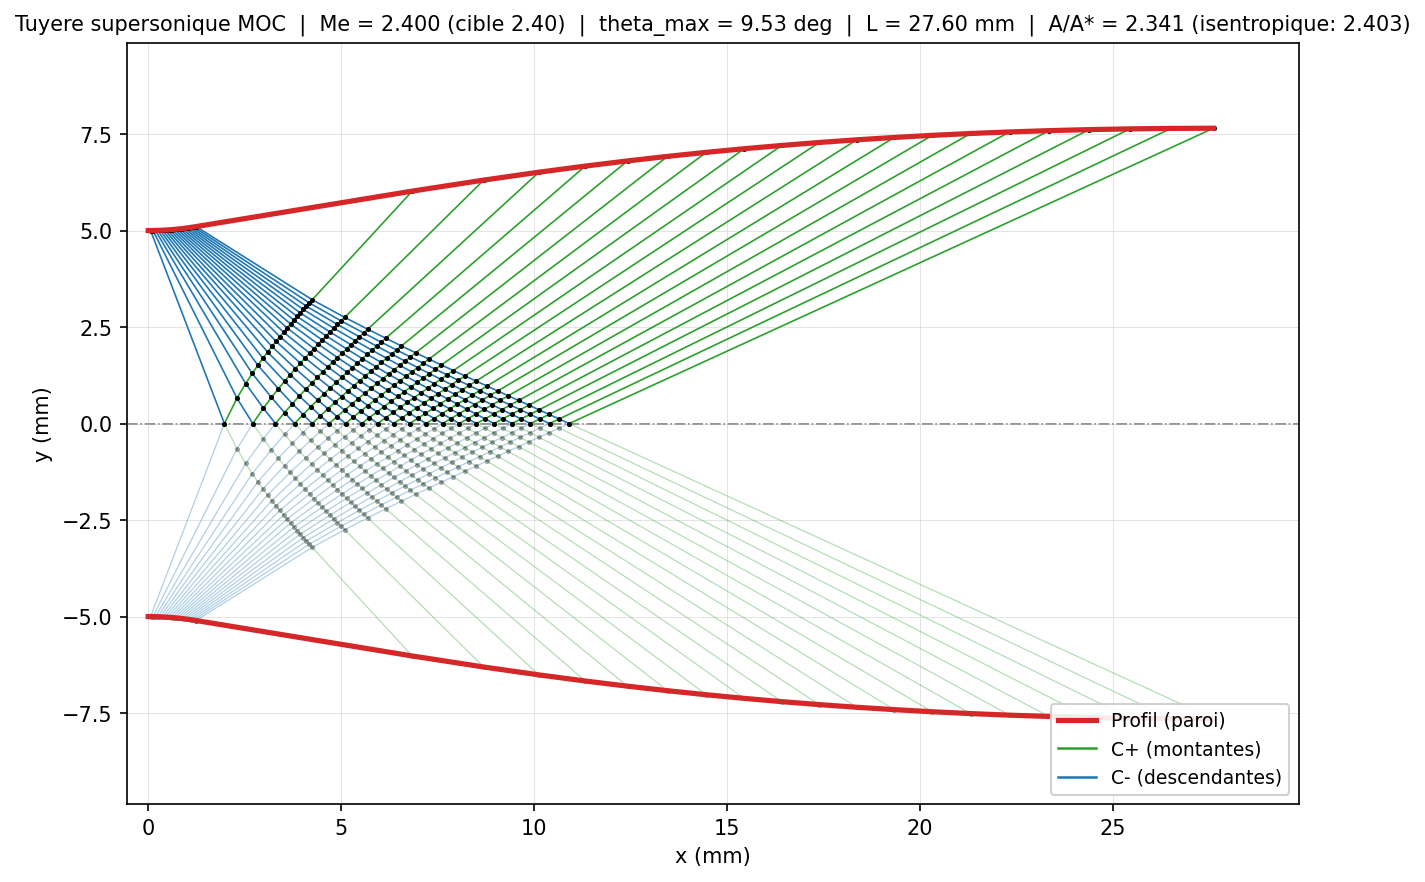
\includegraphics[width=0.95\linewidth]{figures/tuyere_moc.png}
  \caption{Divergent conçu par MOC ($D_{\text{col}}=10$~mm, $M_e=2.4$,
  $\gamma=1.4$, $n=20$)~: profil de paroi (rouge), caractéristiques $C^{+}$
  (vert) et $C^{-}$ (bleu). Le maillage inférieur est le symétrique du
  supérieur.}
  \label{fig:tuyere}
\end{figure}

\begin{table}[H]
  \centering
  \caption{Bilan du cas de référence.}
  \begin{tabular}{lr}
    \toprule
    Grandeur & Valeur \\
    \midrule
    Diamètre du col $D_{\text{col}}$        & $10.0000$ mm \\
    Rayon de l'arc au col $R_c$             & $7.5000$ mm \\
    Mach de sortie visé $M_e$               & $2.4000$ \\
    Mach de sortie obtenu                   & $2.4000$ \\
    Angle de paroi maximal $\theta_{\max}$  & $9.5274^\circ$ \\
    Longueur du divergent                   & $27.6001$ mm \\
    Rayon de sortie $R_{\text{sortie}}$     & $7.6510$ mm \\
    Rapport de sections MOC                 & $2.341495$ \\
    Rapport de sections isentropique        & $2.403100$ \\
    Écart MOC / isentropique                & $-2.564\,\%$ \\
    Nombre total de n\oe uds                   & $251$ \\
    \bottomrule
  \end{tabular}
  \label{tab:bilan}
\end{table}

\section{Limites et précision}
\label{sec:limites}

L'amorçage sur l'arc de cercle repose sur l'\textbf{hypothèse d'onde simple}
($\nu = \theta$) plutôt que sur une analyse transsonique complète du col (ligne
sonique courbe, écoulement rotationnel près de la paroi). Cette approximation
introduit un \textbf{écart systématique d'environ $2$ à $3\,\%$} entre le
rapport de sections calculé par la MOC (éq.~via $(R_{\text{sortie}}/R_t)^2$) et
la valeur isentropique exacte \eqref{eq:hugoniot} --- visible dans la
table~\ref{tab:bilan} ($-2.56\,\%$). Il s'agit d'un \textbf{biais connu et
documenté} de cette méthode de conception, non d'une erreur numérique.

La plage de validation confortable est $M_e \approx 1.5$--$3.5$ pour l'air. Des
Mach de sortie très élevés ou des $\gamma$ proches de $1$ peuvent faire
dégénérer le maillage~; dans ce cas, le code échoue proprement par une
\texttt{ValueError} explicite plutôt que de renvoyer une géométrie aberrante.

\section*{Références}
\addcontentsline{toc}{section}{Références}
\begin{itemize}[nosep]
  \item J. D. Anderson, \emph{Modern Compressible Flow}, chapitre~11
        (Method of Characteristics).
  \item M. J. Zucrow \& J. D. Hoffman, \emph{Gas Dynamics}, vol.~2.
\end{itemize}

\end{document}
